\documentclass[tikz,14pt,fleqn]{article}

% Math
\usepackage[fleqn]{amsmath}
\usepackage{amssymb}
\usepackage{dsfont}
\usepackage{float}

% Insert dummy text
\usepackage{lipsum}  
% Allows to use caption*
\usepackage{caption}
% Scalabale subfigures
\usepackage{subcaption} 
% Code syntax highlighting
\usepackage{minted}
% Hyperlinks
\usepackage{hyperref}
% Customize page layout
\usepackage{geometry}
\geometry{a4paper, margin=1in}
% Page headers and footers
\usepackage{fancyhdr}
\pagestyle{fancy}
\fancyhf{}
\setlength{\parindent}{0pt}
\setlength{\parskip}{0.5\baselineskip}%

% includegraphics
\usepackage{graphicx}




\newcommand{\bmat}[1]{
   \ensuremath{
   \begin{bmatrix}
       #1
   \end{bmatrix}
}}




\usepackage[utf8]{inputenc}


%%%%%%%%%%%%%%%%%%%%%%%%%%%%
%% VARIABLES
\newcommand\namesurname{Albert Cerfeda}
\newcommand\assignment{Assignment 2 - Local Operations}

\newcommand\subject{Image \& Video Processing}
\newcommand\documentdate{20 April 2023}

% Title content
%%%%%%%%%%%%%%%%%%%%%%%%%%%%
\rhead{\assignment}
\lhead{\namesurname}
%%%%%%%%%%%%%%%%%%%%%%%%%%%%

\rfoot{Page \thepage}


\begin{document}

\begin{titlepage}
   \begin{center}
       \vspace*{0.2cm}

       \textbf{\Large{\subject}}

       \vspace{0.5cm}
        \textbf{\assignment}\\[5mm]
        
            
       \vspace{0.4cm}

        \namesurname
        \begin{figure}[H]
            \centering
        \end{figure}
       \tableofcontents

       \vspace*{\fill}
     
        
\includegraphics[width=0.4\textwidth]{fig/logo.png}
       
        \documentdate \\
        Università della Svizzera italiana\\
        Faculty of Informatics\\
        Switzerland\\

   \end{center}
\end{titlepage}

\section{Spatial Filtering [2 points]}

\textbf{Maximum and minimum values of the convoluted image.}

\begin{wrapfigure}{r}{0.25\linewidth}
    \centering
    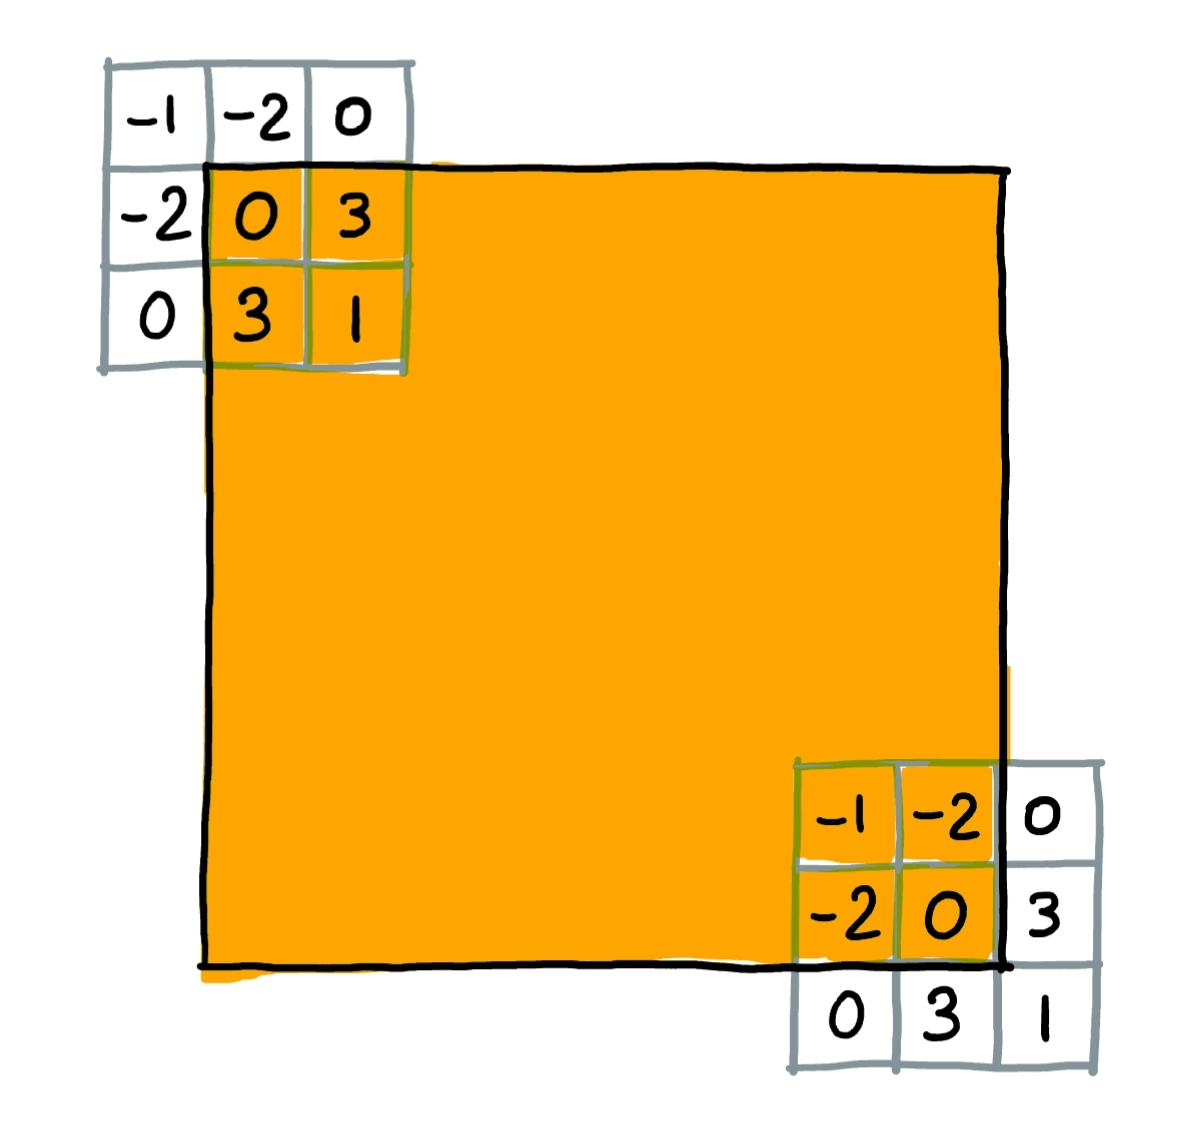
\includegraphics[width=1\linewidth]{fig/1.1.jpg}
    \label{fig:1.1}
\end{wrapfigure}
We know that that each pixel is encoded with in a 6-bit integer format. That is, each pixel has $2^6$ possible values and the minimum and maximum values representable are $0$ and $2^6-1=63$ respectively.\\
To compute the max and min values of the convoluted image, let us consider the case where the filter is getting applied to the corners of the image. Let us employ the padding technique for dealing with pixels outside the bounds of the image (i.e we add artificial pixels with value $0$).\\
If we consider an image where every pixel has value $63$ as a result of the convolution the pixel in the top-left corner will have a value of $(0)*63+(3)*63+(3)*63+(1)*63 = 441$  while the pixel in the bottom-right corner will have a value of $(-1)*63+(-2)*63+(-2)*63+(0)*63 = -315$.

\textbf{Post-filtering pixel transformation.}\\
Knowing that each convoluted pixel ranges from $-315$ to $441$, we can apply a linear transformation to the pixel values. By mapping each pixel intensity by mapping it $x \mapsto (x+315)(\frac{63}{441-(-315)})$ we will map the pixel values to the range $[0,63]$.

\textbf{Separability of filter $H$}\\
For separating a filter we can use the SVD (Singular Value Decomposition) technique\footnote{Singular Value Decomposition (SVD): In linear algebra, the singular value decomposition (SVD) is a factorization of a real or complex matrix. It generalizes the eigendecomposition of a square normal matrix with an orthonormal eigenbasis to any $m\times n$ matrix.[Source \href{https://en.wikipedia.org/wiki/Singular_value_decomposition}{wikipedia.org}]}. The SVD factorizes a matrix $H\in\mathds{R}^{n\times m}$ into:
$$H = U * S * V'$$
where $A$ is an $m \times n$ matrix, $U$ is an $m \times m $orthogonal matrix, $S$ is an $m \times n$ diagonal matrix, and $V$ is an $n \times n$ orthogonal matrix. The diagonal elements of $S$ are the singular values of $A$, which are always non-negative and sorted in decreasing order. The columns of $U$ and $V$ are the left and right singular vectors of $A$, respectively.\\
Let us define $k_1$ and $k_2$ as the row and column vectors into which we will separate filter $H$ into. We can find $k_1$ and $k_2$ by taking the square root of the singular values of $H$ and multiplying them by the corresponding singular vectors.
\vspace{-0.5cm}
\begin{minted}[frame=lines, framesep=2mm, fontsize=\small ]{matlab}
H = [-1 -2 0; -2 0 3; 0 3 1]
[U, S, V] = svd(H)
k1 = sqrt(S(1,1)) * U(:,1)
k2 = sqrt(S(1,1)) * V(:,1)'
\end{minted}
$$
H=\bmat{-1.00&-2.00&0.00\\-2.00&0.00&3.00\\0.00&3.00&1.00}, U=\bmat{-0.27&-0.55&0.79\\0.67&-0.70&-0.25\\0.69&0.46&0.56}, S=\bmat{3.91&0.00&0.00\\0.00&3.55&0.00\\0.00&0.00&0.36}, V=\bmat{-0.27&0.55&-0.79\\0.67&0.70&0.25\\0.69&-0.46&-0.56}
$$
$$
k_1=\bmat{-0.5395\\1.3241\\1.3655}, k_2=\bmat{-0.5395&1.3241&1.3655}
$$
\section{Combining linear operations [2 points]}
We know that the unsharp masking operation can be represented with the following formula:
\begin{figure}[h!]
$$g_{\text {sharp }}=f+\gamma\left(f-h_{\text {blur }} \star f\right)$$
\caption{Unsharp masking operation}
\label{fig:2.1unsharpformula}
\end{figure}\\
i.e we add back to the image the details obtained by subtracting the blurred image from the original image.\\

To compute the kernel reponsible for blurring the image, we can use the Gaussian filter. The gaussian filter computes a weighted average of the pixels in the neighborhood. The weights fall off as the distance increases from the center pixel, according to the gaussian distribution. We can control such gaussian distribution by changing the value of the standard deviation $\sigma$ (i.e control the amount of blur). The size for the kernel matters: to give a good approximated representation of the gaussian function we choose the kernel size to be $4\sigma +1$.\\

We notice how we can translate the unsharp masking operation [Figure \ref{fig:2.1unsharpformula}] into a linear operation between kernels [Figure \ref{fig:2.2}]. Notice how the kernel for the original image is just a zero matrix with a $1$ in the center. The kernel for the blurred image is the gaussian filter. The difference between the two kernels is the image details.\\
Parameter $\gamma$ serves as a control parameter for determining the amount of sharpening.\\The code for computing the unsharp masking kernel is rather simple [Figure \ref{fig:2.3code}]. Notice how ideally more details would have been extracted with a higher $\sigma$ value. It has been kept purposefully low for generating small matrices, in order to fit them in the report. The results are shown in [Figure \ref{fig:2.4}].
\begin{figure}[h!]
    \begin{subfigure}[b]{\linewidth}
    $$\bmat{0&0&0&0&0\\0&0&0&0&0\\0&0&1&0&0\\0&0&0&0&0\\0&0&0&0&0} + \gamma  \underbrace{\pmat{\underbrace{\bmat{0&0&0&0&0\\0&0&0&0&0\\0&0&1&0&0\\0&0&0&0&0\\0&0&0&0&0}}_{\text{Original pixel}} - \underbrace{\bmat{0.00&0.01&0.02&0.01&0.00\\0.01&0.06&0.10&0.06&0.01\\0.02&0.10&0.16&0.10&0.02\\0.01&0.06&0.10&0.06&0.01\\0.00&0.01&0.02&0.01&0.00}}_{\text{Blurred pixel}}}}_{\text{Image details}} $$
    \caption[]{Kernel computation for unsharp masking.\\$\sigma=1, \gamma = 8$}
    \end{subfigure}
    \begin{subfigure}[b]{\linewidth}
        $$\bmat{-0.02&-0.11&-0.18&-0.11&-0.02\\-0.11&-0.48&-0.79&-0.48&-0.11\\-0.18&-0.79&7.70&-0.79&-0.18\\-0.11&-0.48&-0.79&-0.48&-0.11\\-0.02&-0.11&-0.18&-0.11&-0.02} $$
        \caption[]{Resulting unsharp masking kernel}
    \end{subfigure}
    \caption{Computing the unsharp masking kernel}
    \label{fig:2.2}
\end{figure}
\begin{figure}[h!]
    \begin{minted}[frame=lines, framesep=2mm, fontsize=\small ]{matlab} 
% ...
% Create gaussian blur filter with a gamma parameter of 1
sigma = 1;
gamma = 8;
size = 4*sigma + 1;
blur_f = fspecial('gaussian', size, sigma);
% Identity kernel - leaves the pixel untouched
identity_f = zeros(size);
identity_f(ceil(size/2), ceil(size/2)) = 1;
% Unsharp filter
unsharp_filter = identity_f + gamma.*(identity_f - blur_f);
im_sharp = imfilter(im, unsharp_filter);
\end{minted}
\caption{Matlab code computing the unsharp masking kernel.}
\label{fig:2.3code}
\end{figure}

\begin{figure}[h!]
    \begin{subfigure}[b]{0.5\linewidth}
        \centering
    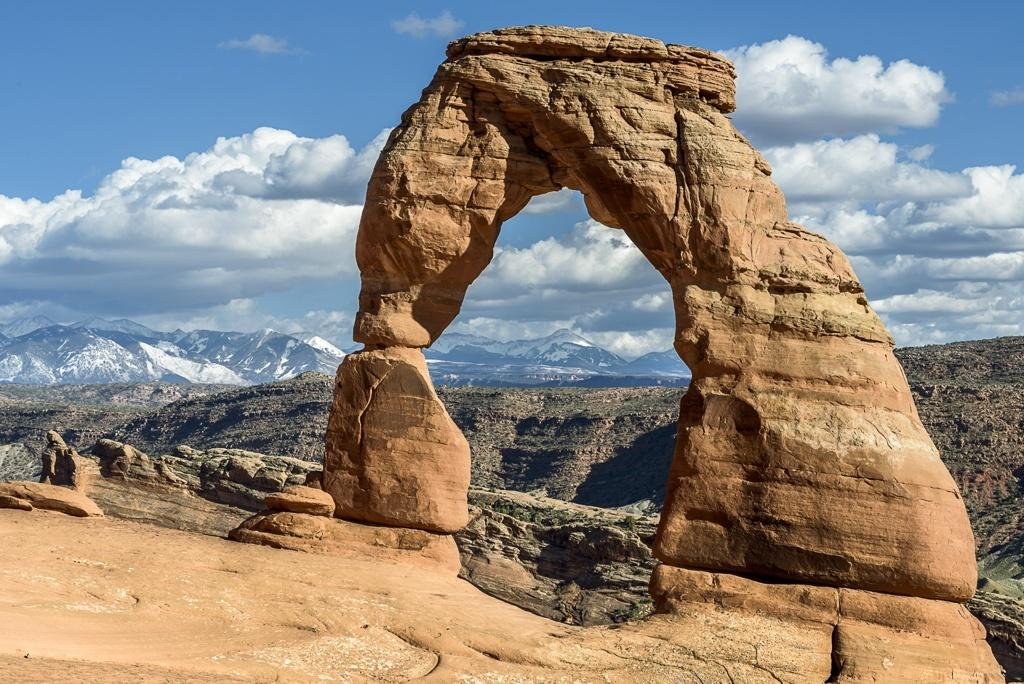
\includegraphics[width=0.7\linewidth]{fig/out/2.im.jpg}
    \caption{Original image}
    \end{subfigure}
    \begin{subfigure}[b]{0.5\linewidth}
        \centering
        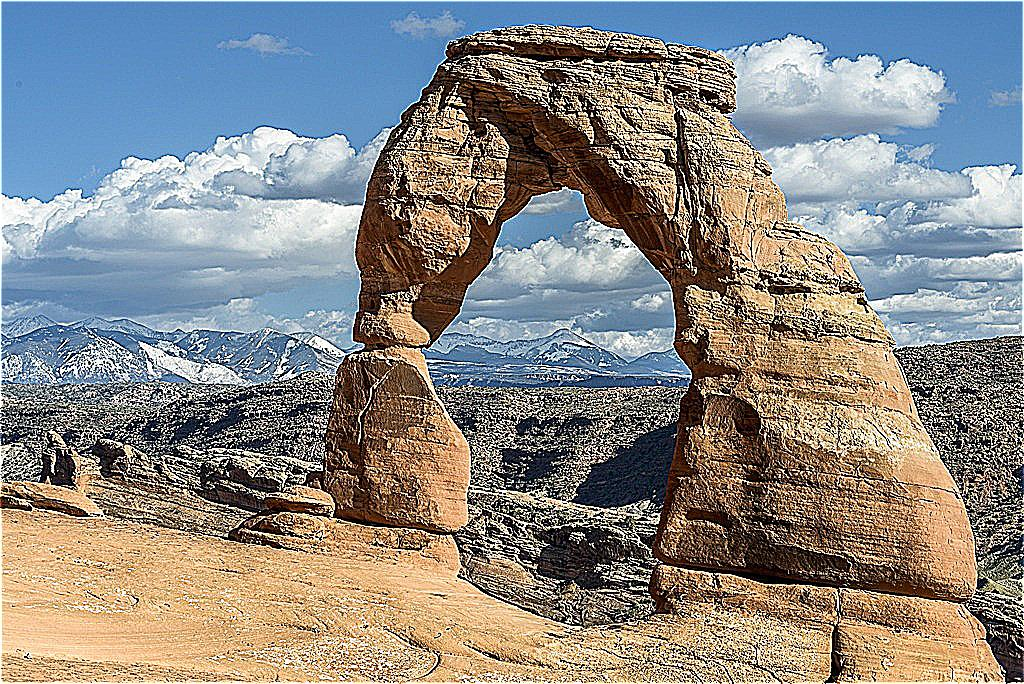
\includegraphics[width=0.7\linewidth]{fig/out/2.im_sharp.jpg}
        \caption{Sharpened image}
    \end{subfigure}
    \caption{Unsharp masking results.}
    \label{fig:2.4}
\end{figure}
\section{Morphological operations A [2 points]}
Morphological operations are a set of operations that are applied to binary images, in order to alter the represented shapes.\\
The exercise requires to choose one structuring element and perform multiple morphological operations on the binary image in order to obtain the desired result.\\
By choosing structural element $c)$ we can obtain the desired result by performing erosion and dilation in succession. Results are shown in Figure \ref{fig:3}:
\begin{figure}[h!]
    \begin{subfigure}[b]{0.33\linewidth}
        \centering
    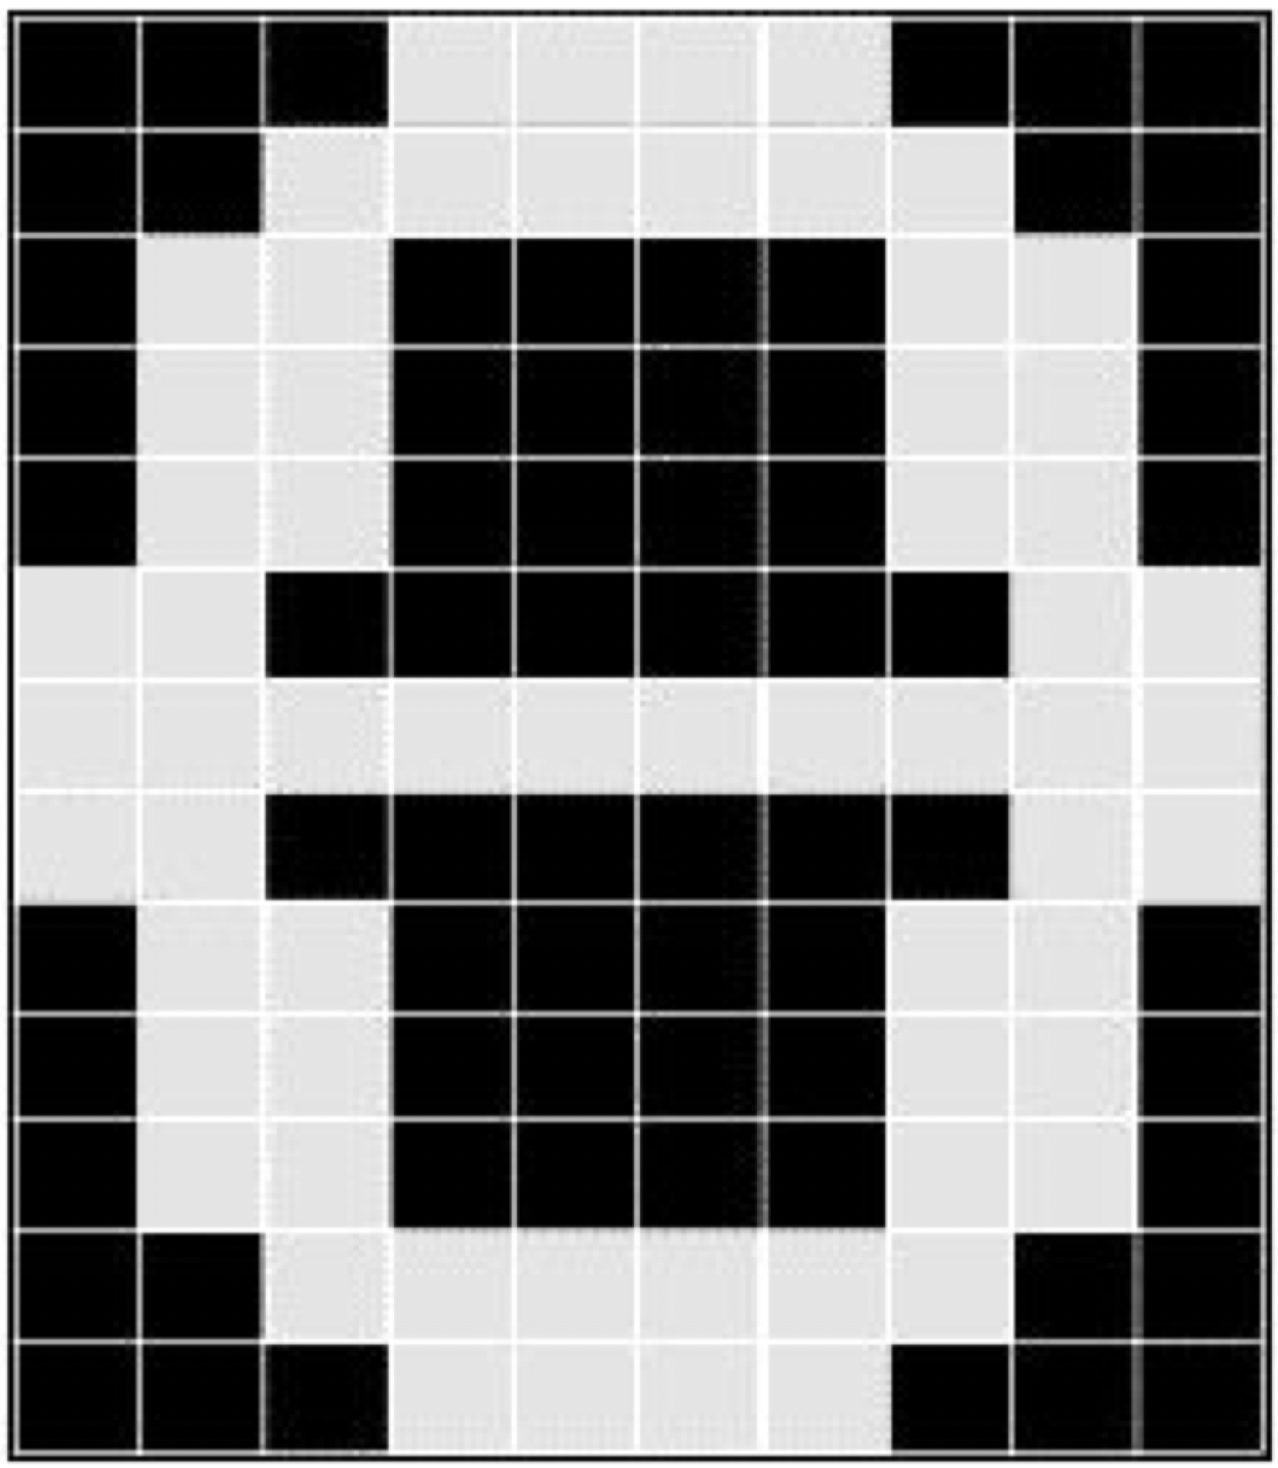
\includegraphics[width=.5\linewidth]{fig/3.0.png}
    \caption{Original binary image}
    \end{subfigure}
    \begin{subfigure}[b]{0.33\linewidth}
        \centering
        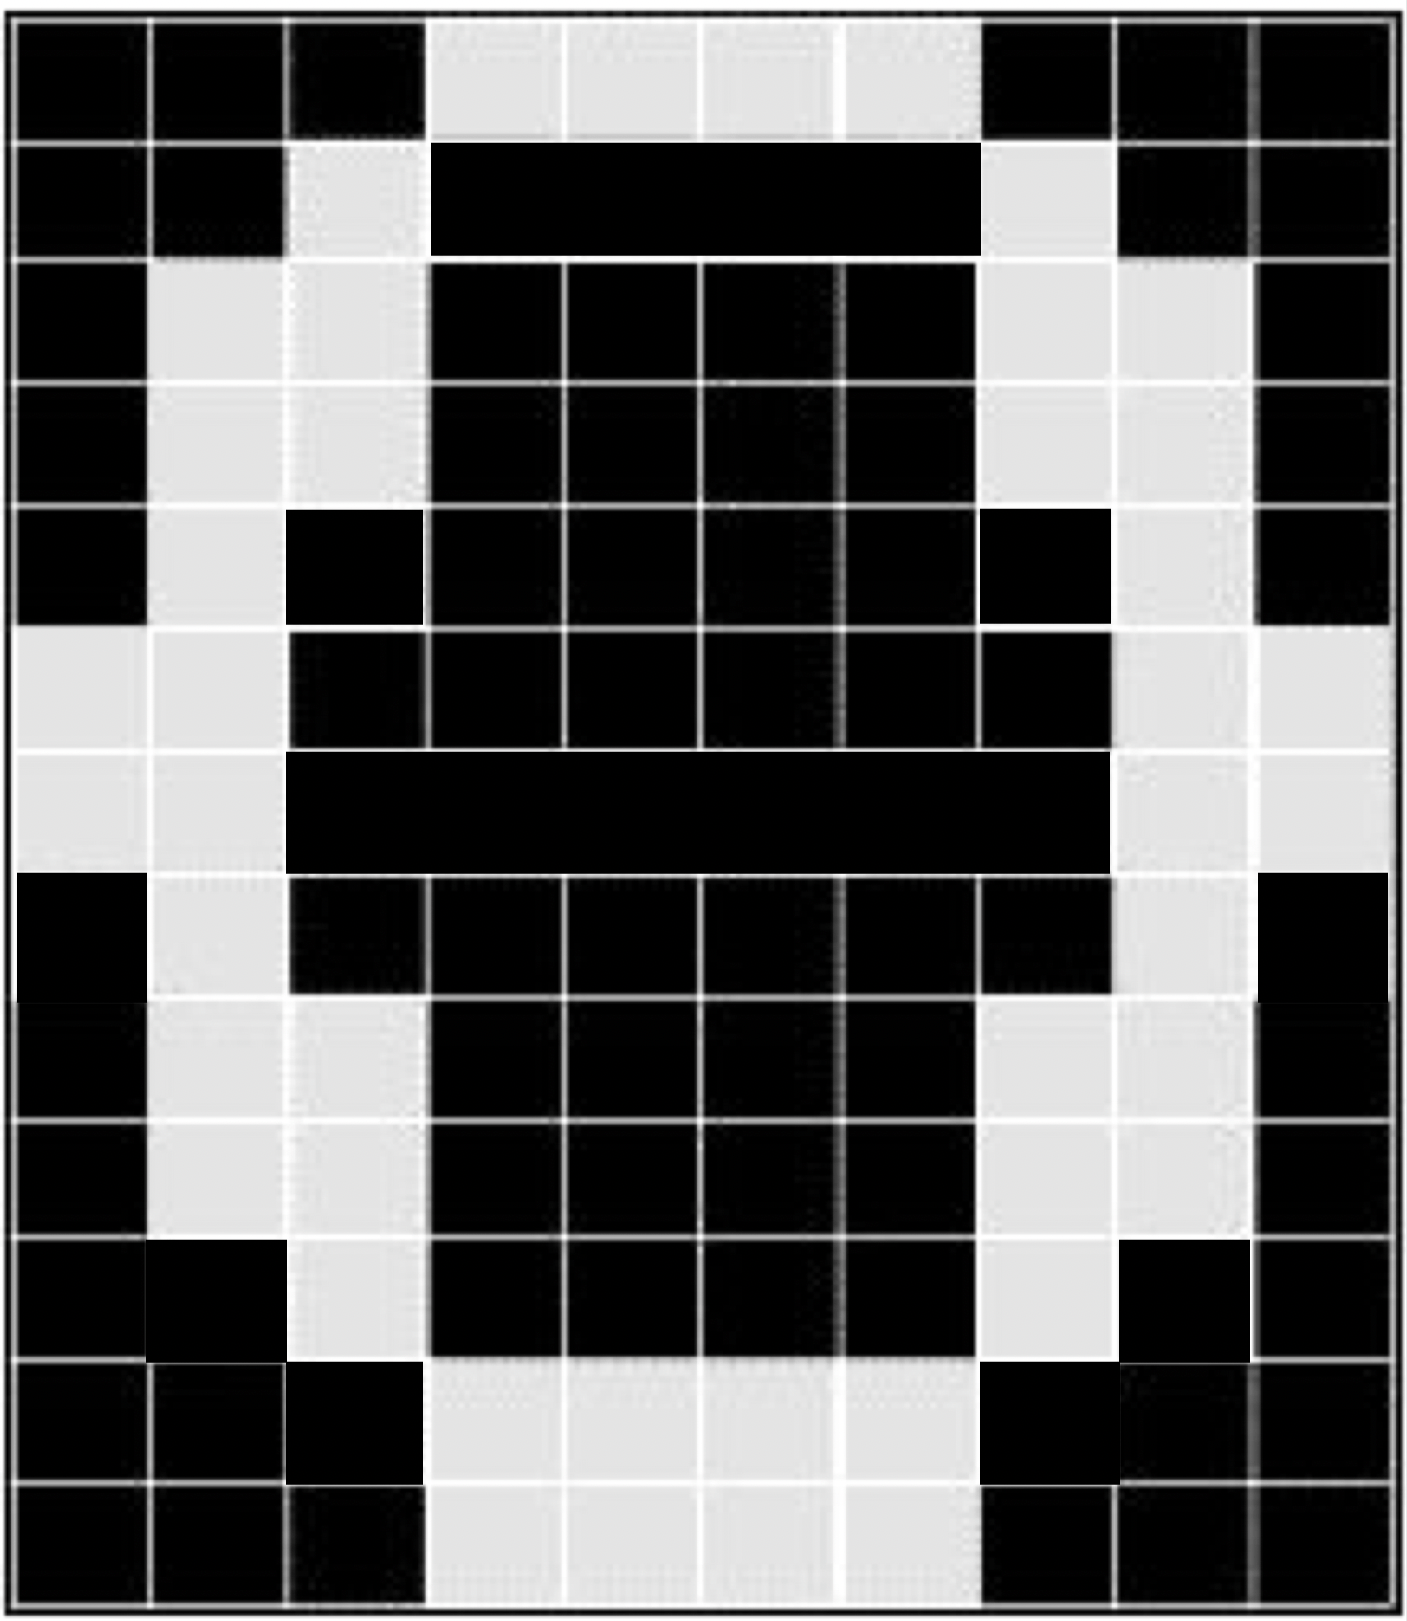
\includegraphics[width=.5\linewidth]{fig/3.1.png}
        \caption{Erosion}
    \end{subfigure}
    \begin{subfigure}[b]{0.33\linewidth}
        \centering
        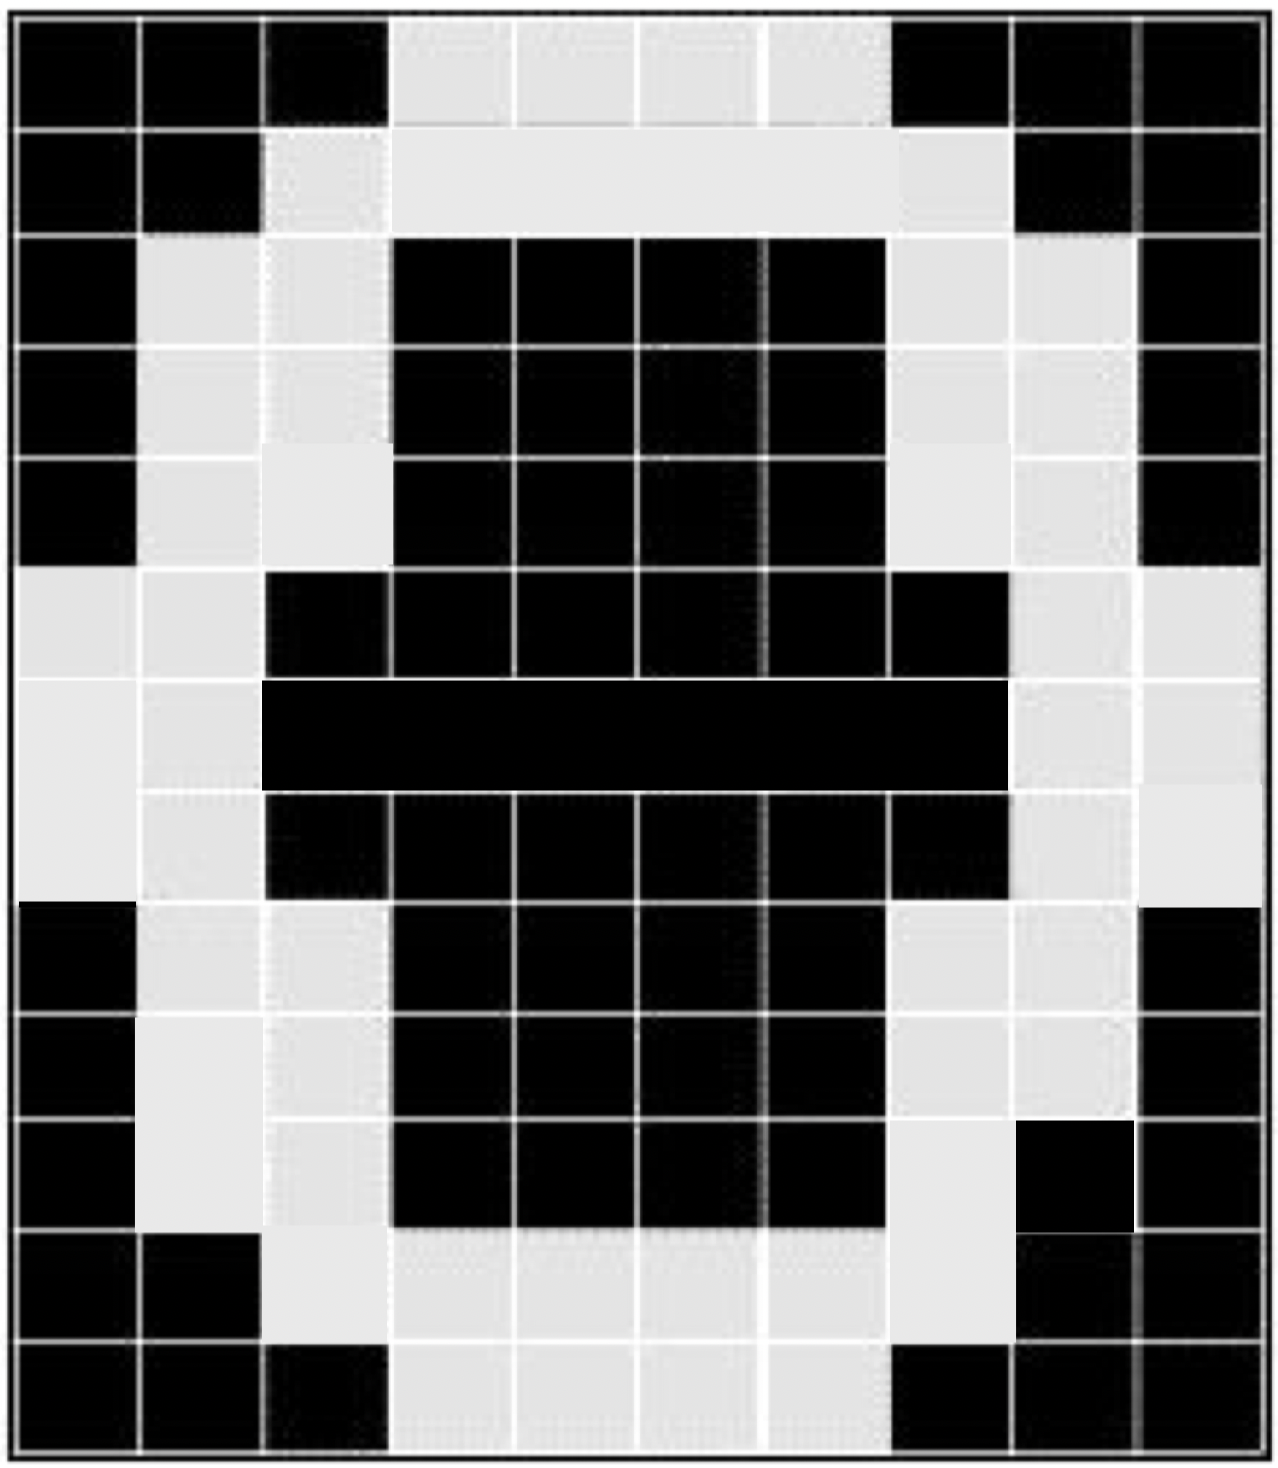
\includegraphics[width=.5\linewidth]{fig/3.2.png}
        \caption{Erosion + Dilation}
    \end{subfigure}
    \caption{Morphological operations using structuring element c)}
    \label{fig:3}
\end{figure}
\section{Morphological operations B [2 points]}
Having just one foreground pixel in the structuring element and applying erosion on a binary image results in the removal of the edges in a particular direction.\\
It can be easily visualized by thinking of shining a directed light on the shape, and by eroding the pixels that are in shadow. The farther the white pixel in the structuring element is from the target pixel, the greater the "shadow" is. The demonstration is shown in Figure \ref{fig:4}:
\begin{figure}[h!]
    \begin{subfigure}[b]{0.195\linewidth}
        \centering
        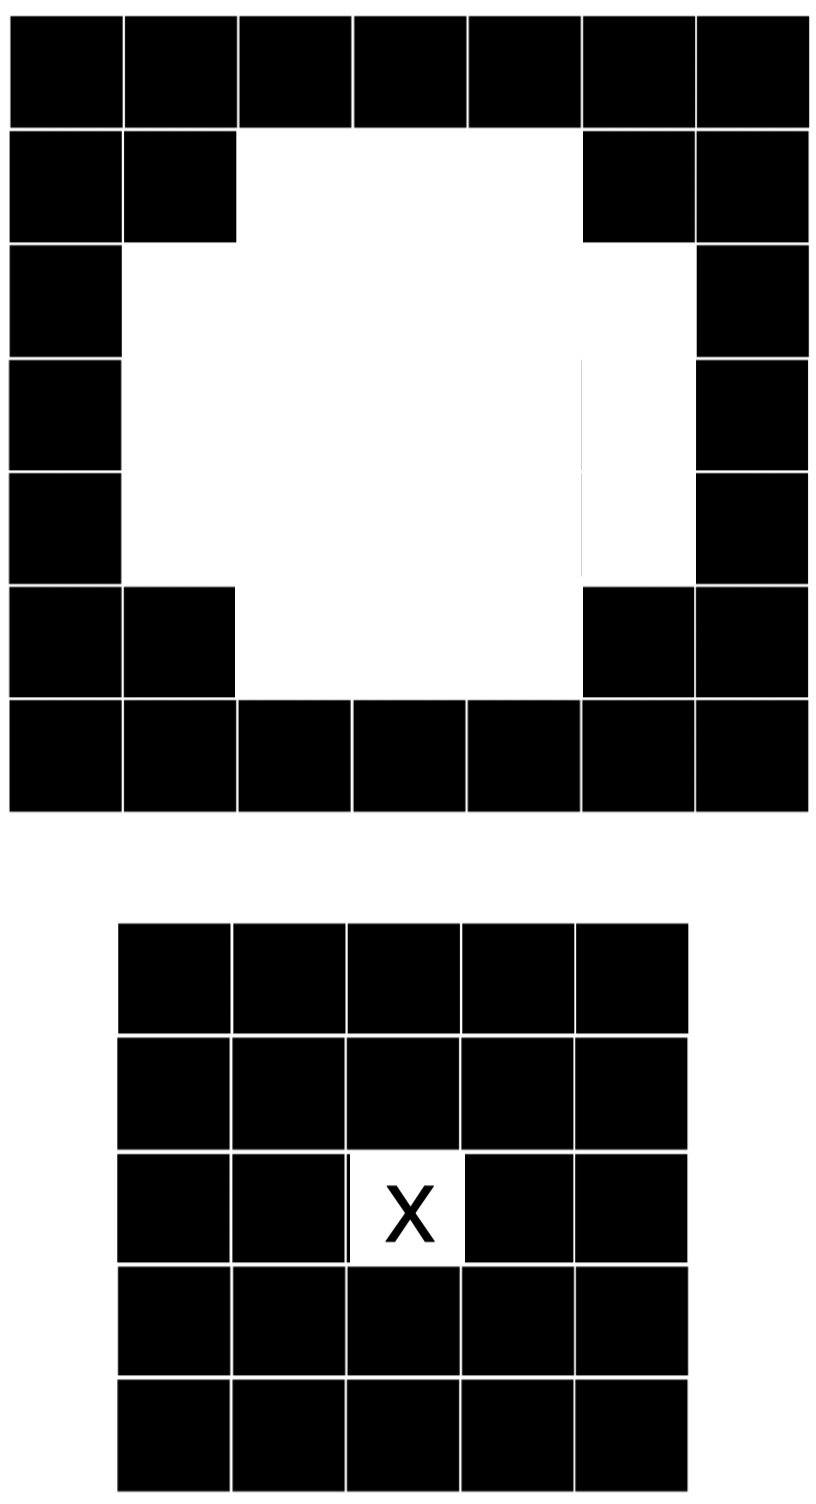
\includegraphics[width=\linewidth]{fig/4.er1.png}
    \end{subfigure}
    \begin{subfigure}[b]{0.195\linewidth}
        \centering
        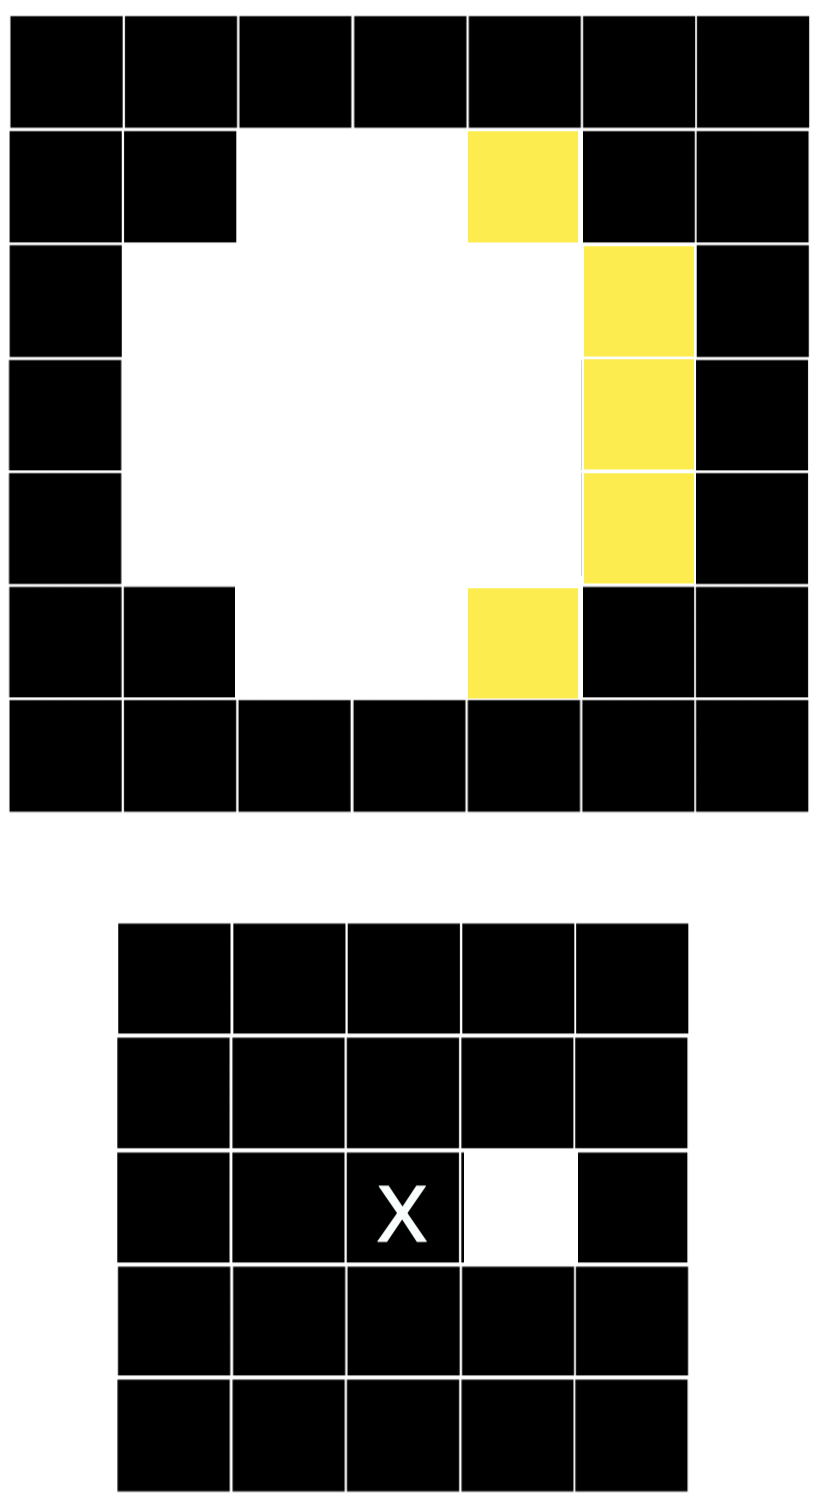
\includegraphics[width=\linewidth]{fig/4.er2.png}
    \end{subfigure}
    \begin{subfigure}[b]{0.195\linewidth}
        \centering
        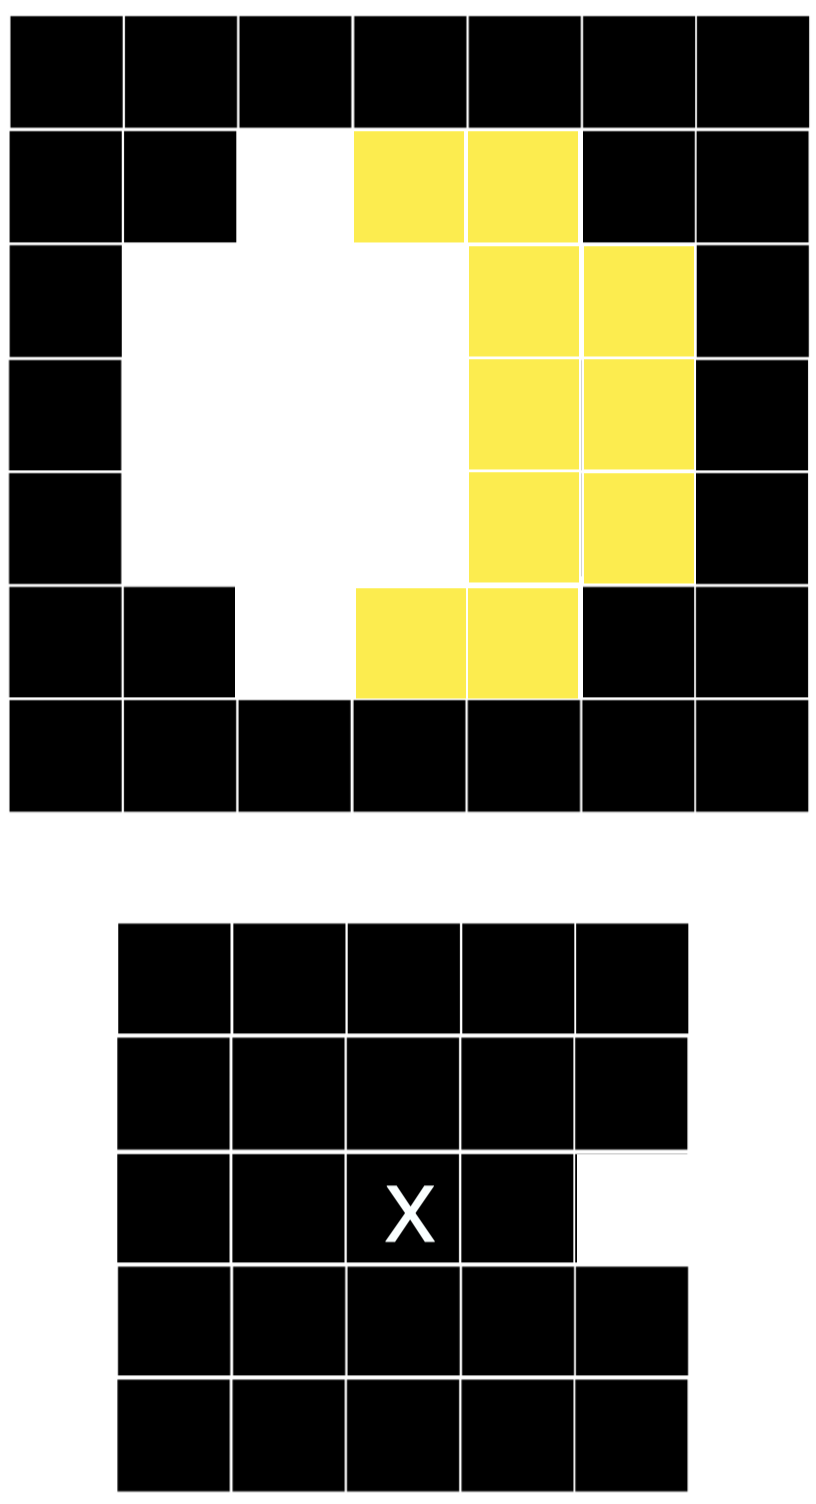
\includegraphics[width=\linewidth]{fig/4.er3.png}
    \end{subfigure}
    \begin{subfigure}[b]{0.195\linewidth}
        \centering
        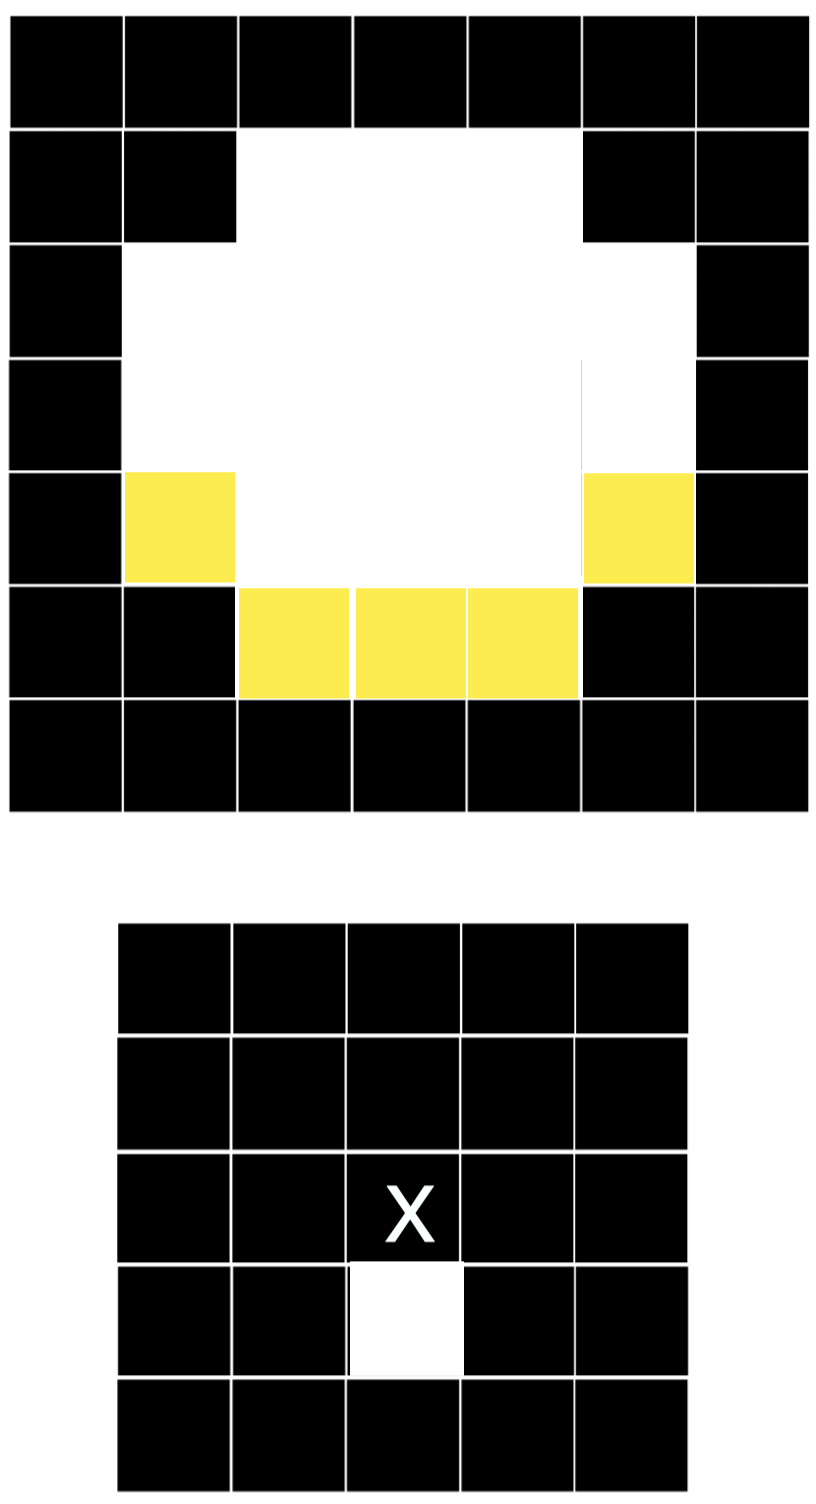
\includegraphics[width=\linewidth]{fig/4.er4.png}
    \end{subfigure}
    \begin{subfigure}[b]{0.195\linewidth}
        \centering
        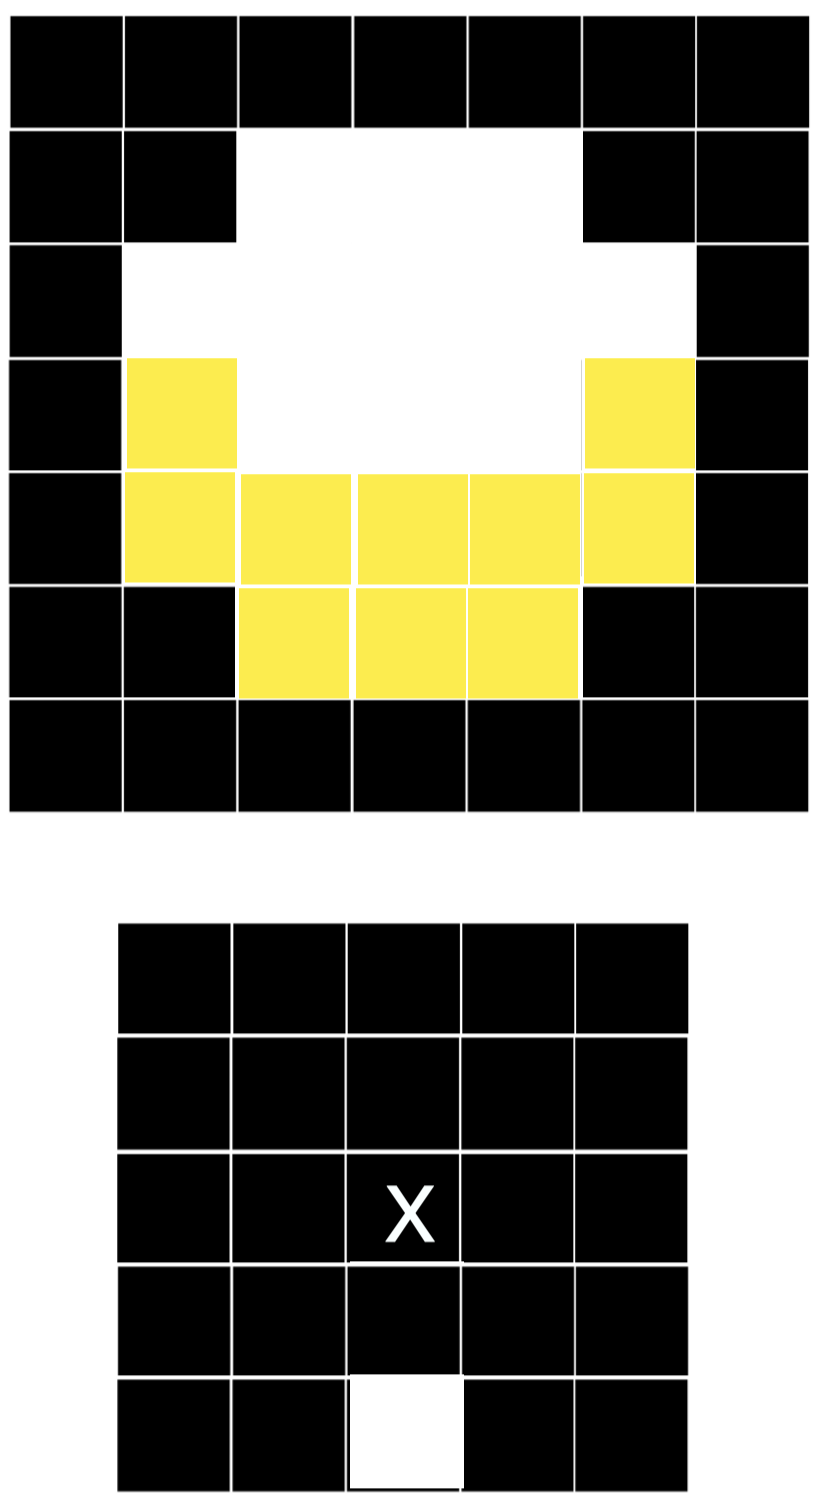
\includegraphics[width=\linewidth]{fig/4.er5.png}
    \end{subfigure}
    \caption{Erosion comparison for arbitrary structuring elements}
    \label{fig:4}
\end{figure}
\section{Linear Motion Blur Filter [4 points]}
The gaussian function is the same on every axis i.e it falls off equally in every direction. However, in the case of motion blur, each axis can have a separate gaussian function. This allows us to mimic the effect of motion blur.\\
Additionally, we want to provide the angle in degrees for which we rotate the kernel. Let us implement function \mintinline{matlab}{gaussianKernel(sigma,angle)} for computing the anisotropic gaussian kernel.
\begin{figure}[h!]
\begin{minted}[ frame=lines, framesep=2mm, linenos, fontsize=\small ]{matlab} 
function res = gaussianKernel(sigma, angle)
    if size(sigma) == 1
        sigma = [sigma, sigma];
    end
    angle = deg2rad(angle);
    kernelsize = 4*sigma+1;
    kernelsize = abs([cos(angle) sin(angle)]) .* kernelsize(1) + abs([sin(angle) cos(angle)]) .* kernelsize(2);

    [X,Y] = meshgrid(1:kernelsize(2),1:kernelsize(1));
    X = X - kernelsize(2)/2; 
    Y = Y - kernelsize(1)/2;
    Xg = X * cos(angle) - Y * sin(angle);
    Yg = X * sin(angle) + Y * cos(angle);

    res = exp(-(Xg.^2/(2*sigma(2)^2) + Yg.^2/(2*sigma(1)^2)));
    res = res / sum(res(:));
end
\end{minted}
\caption{Matlab function for computing an anisotropic gaussian kernel.}
\end{figure}

We can call the function like so:
\vspace*{-0.5cm}
\begin{minted}[frame=lines, framesep=2mm]{matlab} 
gaussianKernel([10, 1], -45)
\end{minted}
\vspace*{-0.5cm}
The function will return a gaussian kernel with $\sigma^y=10, \sigma^x=1,\theta=-45\degree$ i.e a standard deviation of $10$ in the $y$ direction and $1$ in the $x$ direction. Finally the kernel will be rotated by $-45$ degrees. [Results are shown in Figure \ref{fig:5.3}]\\\\
A regular isotropic gaussian kernel with $\sigma=5$ can be obtained in the following way [Results are shown in Figure \ref{fig:5.2}]:
\vspace*{-0.5cm}
\begin{minted}[frame=lines, framesep=2mm]{matlab} 
gaussianKernel(5, 0)
\end{minted}
The function derives the optimal kernel size for the given $\theta,\sigma^x\text{ and }\sigma^y$. It first creates a non-rotated kernel with size $\bmat{4*\sigma^x+1 & 4*\sigma^y+1}$ after which a "bounding box" containing the rotated kernel is created. This bounding box is then afterwards populated with the kernel values.\\
\vspace*{-0.5cm}
\begin{figure}[h!]
    \centering
    \begin{subfigure}[b]{0.28\linewidth}
        \centering
        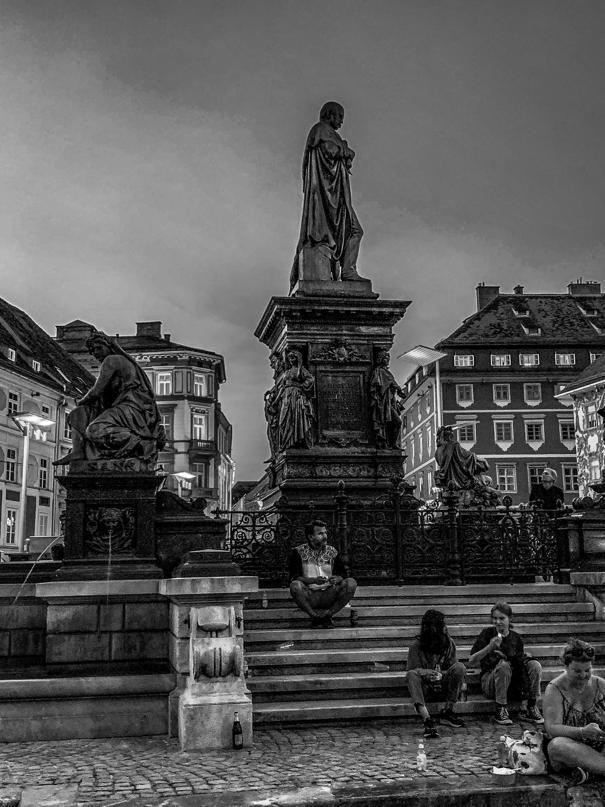
\includegraphics[width=\linewidth]{fig/out/5.im.jpg}
        \phantom{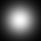
\includegraphics[width=.4\linewidth]{fig/out/5.blur_filter.jpg}}
        \caption{Original image\\$\sigma=0$}
        \label{fig:5.1}
    \end{subfigure}
    \begin{subfigure}[b]{0.28\linewidth}
        \centering
        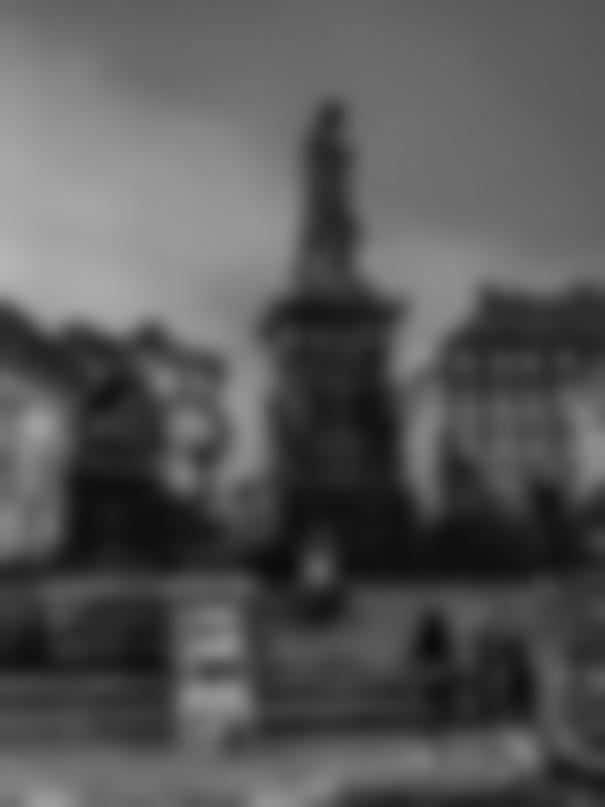
\includegraphics[width=\linewidth]{fig/out/5.im_blur.jpg}
        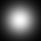
\includegraphics[width=.4\linewidth]{fig/out/5.blur_filter.jpg}
        \caption{Regular isotropic gaussian blur\\$\sigma=5$}
        \label{fig:5.2}
    \end{subfigure}
    \begin{subfigure}[b]{0.28\linewidth}
        \centering
        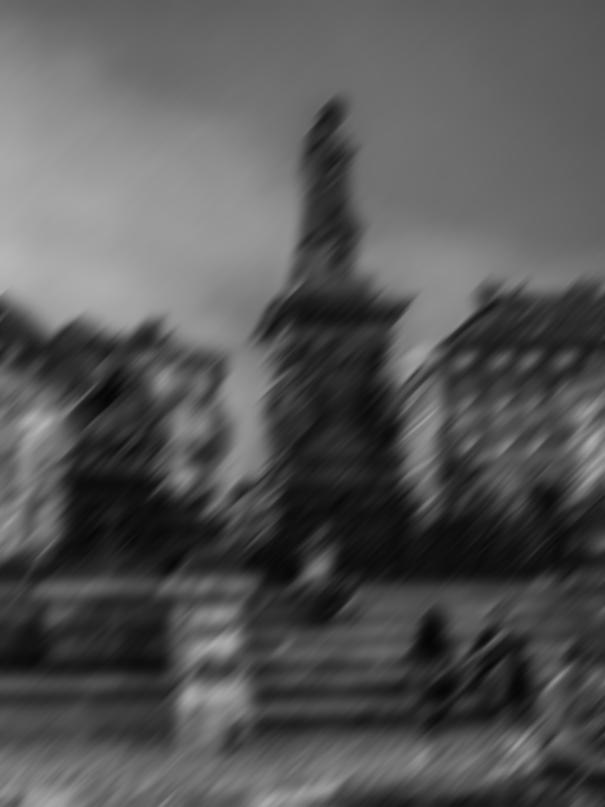
\includegraphics[width=\linewidth]{fig/out/5.im_motionblur.jpg}
        
\includegraphics[width=.4\linewidth]{fig/out/5.motionblur_filter.jpg}
        \caption{Anisotropic gaussian blur\\$\sigma^y=10, \sigma^x=1,\theta=-45\degree$}
        \label{fig:5.3}
    \end{subfigure}
    \caption{Gaussian kernel comparison}
    \label{fig:5}
\end{figure}

\section{Iterative filtering [4 points]}
Iterative filtering consists in approximating a bigger kernel filter by repeatedly applying a smaller kernel filter.\\
In the case of Gaussian blur, we can perform iterative filtering to approximate a bigger Gaussian kernel.\\
Gaussian filtering assigns the weights for each pixel based solely on spatial distance. We can intuitevely infer that since the distances between pixels stay the same, if we repeatedly apply a smaller Gaussian filter, the pixel values will eventually converge to the same values as if we had applied a bigger Gaussian filter.\\\\
Bilateral filtering additionally takes into consideration the color difference between pixels when assigning weights in order to preserve edges. As the pixel values change for each iteration, the color difference between pixels will also change. Therefore, we can not expect the pixel values to converge to the same values as if we had applied a bigger bilateral filter.\\\\
When inspecting an image obtained through iterative filtering with bilateral filtering, we also notice how there is an increase in aliasing artifacts. The cause for the effect is may due to the fact that by repeatedly applying the filter, a greater degree of smoothing is applied resulting in a loss of details. Additionally the bilateral filter tries to preserve edges. This results in sharper edges with a possible increase of aliasing artefacts. Results are shown in Figure \ref{fig:6.3}.
\vspace*{-0.5cm}
\begin{minted}[frame=lines, framesep=2mm, fontsize=\small ]{matlab} 
% ...
% Edge preserving bilateral filtering
im_bilat = imbilatfilt(im, 0.12, 6);
im_bilat2 = im;
for i = 1:45
    im_bilat2 = imbilatfilt(im_bilat2, 0.012, 0.6);
end
\end{minted}
\vspace*{-0.5cm}

\begin{figure}[h!]
    \centering
    \begin{subfigure}[b]{0.325\linewidth}
        \centering
        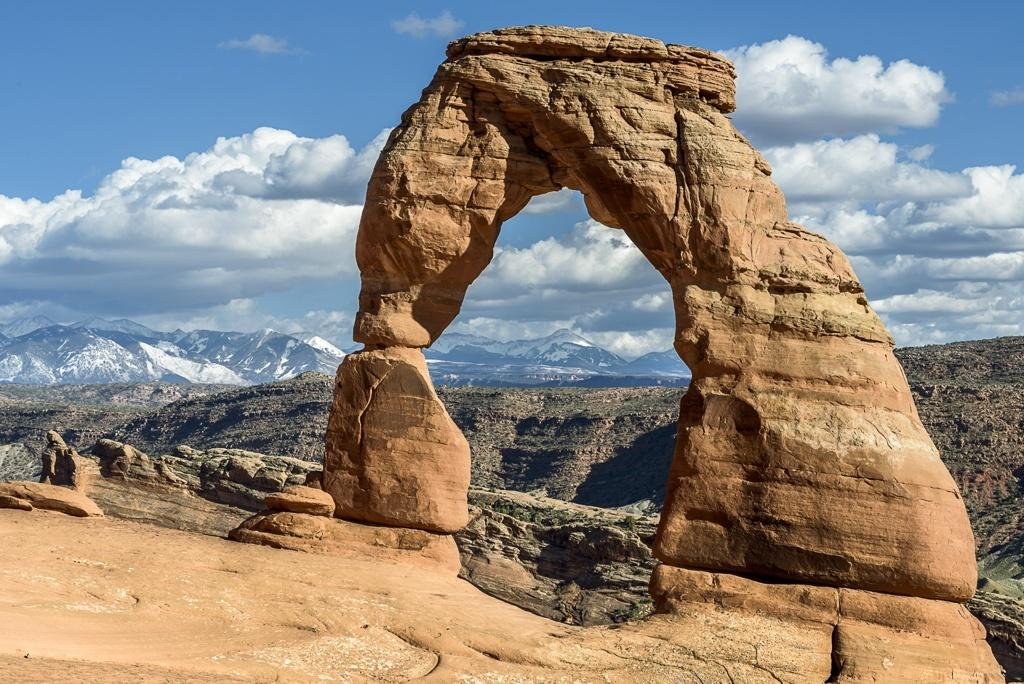
\includegraphics[width=\linewidth]{fig/out/6.im.jpg}
        \caption{Original image}
    \end{subfigure}
    \begin{subfigure}[b]{0.325\linewidth}
        \centering
        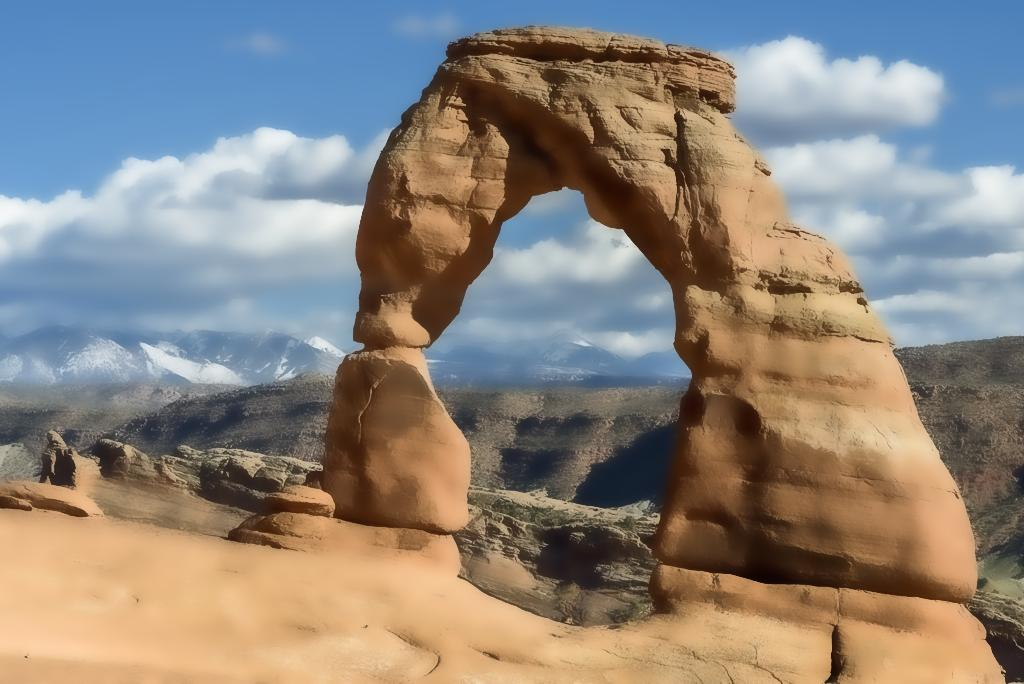
\includegraphics[width=\linewidth]{fig/out/6.im_bilat.jpg}
        \caption{\mintinline{matlab}{imbilatfilt(im,0.12,6)}}
    \end{subfigure}
    \begin{subfigure}[b]{0.325\linewidth}
        \centering
        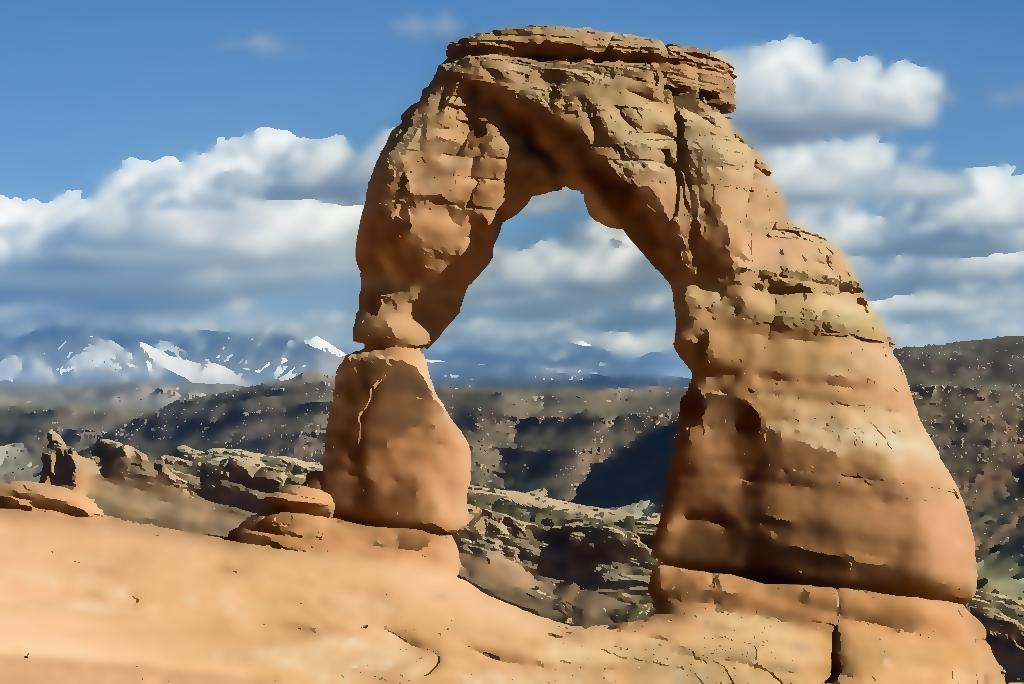
\includegraphics[width=\linewidth]{fig/out/6.im_bilat2.jpg}
        \caption{45x \mintinline{matlab}{imbilatfilt(im,0.012,0.6)}}
        \label{fig:6.3}
    \end{subfigure}
    \caption{Gaussian kernel comparison}
    \label{fig:6}
\end{figure}


\subsection{Image Stylization [4 points]}
\begin{wrapfigure}{r}{0.23\linewidth}
    \centering
    \vspace*{-0.5cm}
    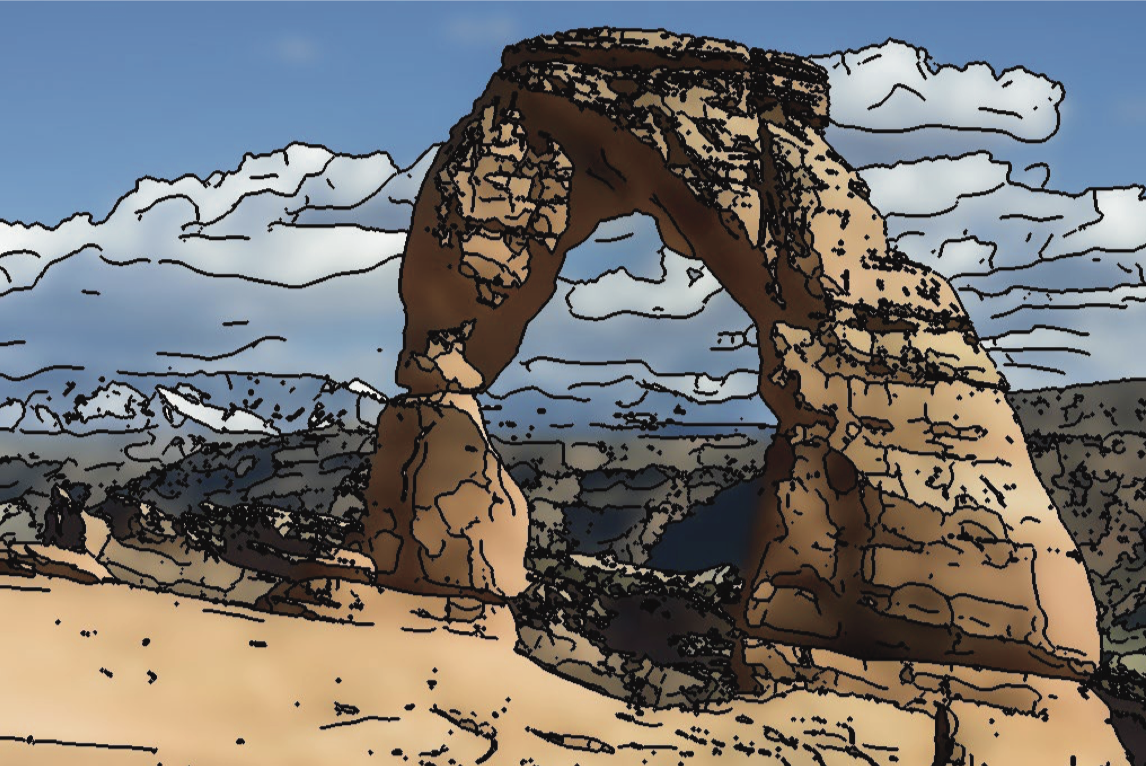
\includegraphics[width=1\linewidth]{fig/6.1.goal.png}
    \label{fig:1.1}
\end{wrapfigure}
We are tasked in stylizing the image and mimic the appearance of the provided image. There are two noticeable effects present in the stylized image:
\begin{itemize}
    \item The underlying image is blurred
    \item The edges of the image content are thickened and blackened
\end{itemize}
Let us implement the code for performing such stylization on image \verb|delicate_arch.jpg|:
\vspace*{-1cm}
\begin{minted}[frame=lines, framesep=2mm]{matlab}
% 1. Find edges using Canny algorithm
im_bilat = imbilatfilt(im, 0.9, 6);
edges = edge(rgb2gray(im_bilat), 'canny');

% 2. Dilate edges
edges = imdilate(edges, strel('disk', 2));

% 3. Use the edges as a mask to stylize the image
im_stylized = im_bilat.*~edges;
\end{minted}
Notice how the Canny\footnote{Canny edge detection: Uses linear filtering with a Gaussian kernel to smooth noise and then computes the edge strength and direction for each pixel in the smoothed image. [Sources \href{https://indiantechwarrior.com/canny-edge-detection-for-image-processing/}{indiantechwarrior.com}, \href{https://ch.mathworks.com/help/images/ref/edge.html}{mathworks.com}]} algorithm has been used for computing the edges of the image. In my experience using the Canny algorithm yields the best results, as it tends to group regions of similar color values together, resulting in the desired cartoonish effect.

\begin{figure}[h!]
    \centering
    \begin{subfigure}[b]{0.325\linewidth}
        \centering
        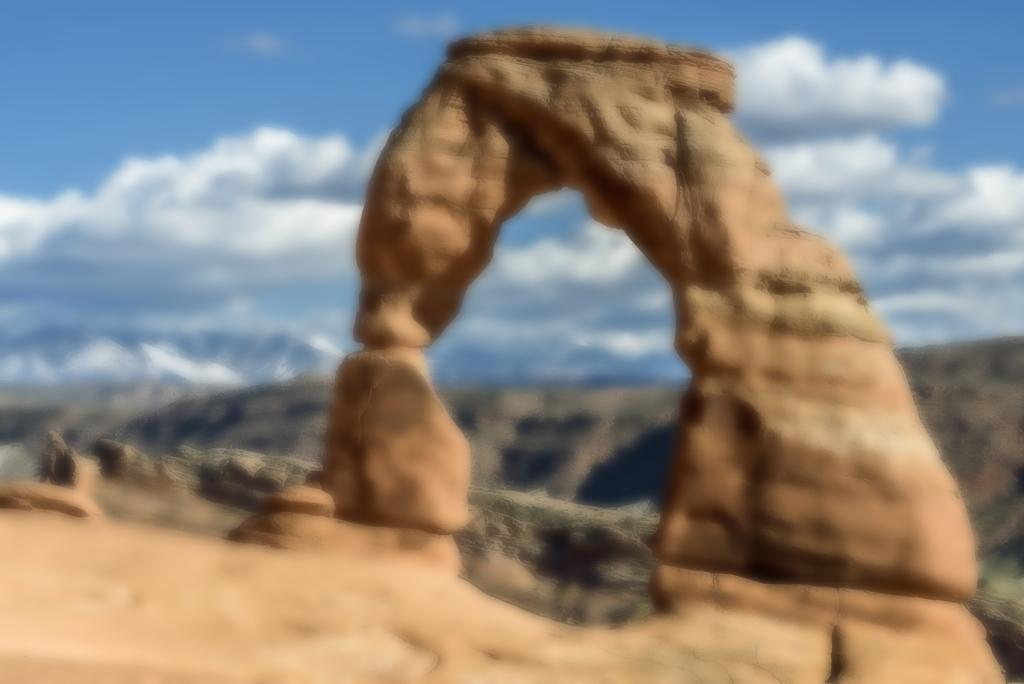
\includegraphics[width=\linewidth]{fig/out/6.1.im_bilat.jpg}
        \caption{Bilateral blurred image}
    \end{subfigure}
    \begin{subfigure}[b]{0.325\linewidth}
        \centering
        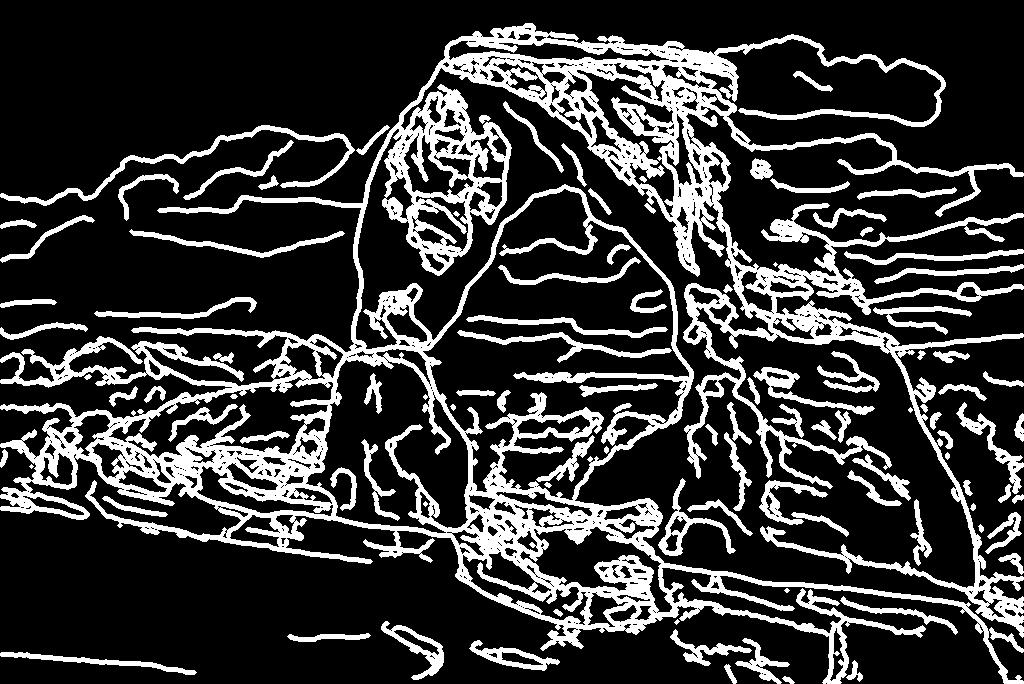
\includegraphics[width=\linewidth]{fig/out/6.1.im_bilat_edges.jpg}
        \caption{Edges}
    \end{subfigure}
    \begin{subfigure}[b]{0.325\linewidth}
        \centering
        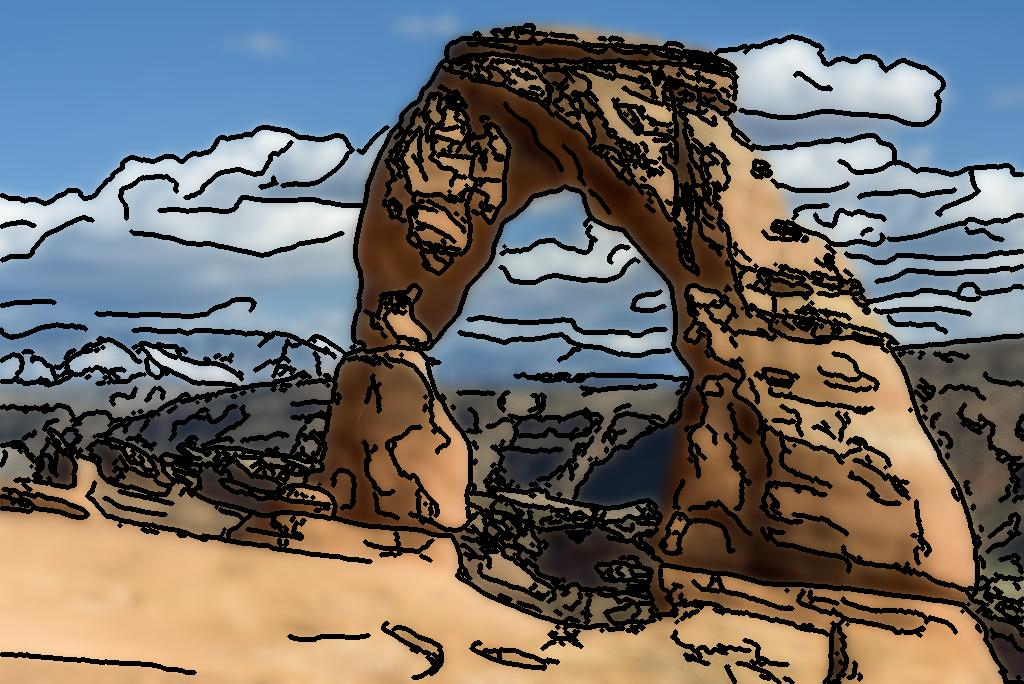
\includegraphics[width=\linewidth]{fig/out/6.1.im_stylized.jpg}
        \caption{Final sytlized image}
    \end{subfigure}
\end{figure}


\end{document}